\chapter{Case Study}
In this part of the thesis, we will be attempting to control the Furuta pendulum. The main control goal is the swing-up control of the pendulum. It means, that initially, the pendulum is steady at the downside position, and we are aiming to bring it to the upright position, and stabilize it there. There are two ways to achieve that, the heuristic swing-up control strategy and optimal swing-up control strategy, which are described in Section \ref{Hswing:teoria}  and Section \ref{nmpcsection} respectively. Those two strategies are applied to control the pendulum device, which is represented by its non-linear dynamic model~\ref{nonlinmodel}. After, the achieved results will be compared and discussed.
\section{Laboratory Furuta Pendulum Device}
Before any control strategy can be developed, the controlled object must be studied. The mathematical representation of the Furuta pendulum was derived in Section~\ref{furuta_Theory} in a form of linear and non-linear dynamic models. In those models appears the physical parameters of the device (Tab.~\ref{furuta:params}). As the pendulum device is available in the laboratory (Fig.~\ref{furutareal}), there is no need to estimate those parameters, but the can be directly measured.
\begin{figure}[H]
	\centering
	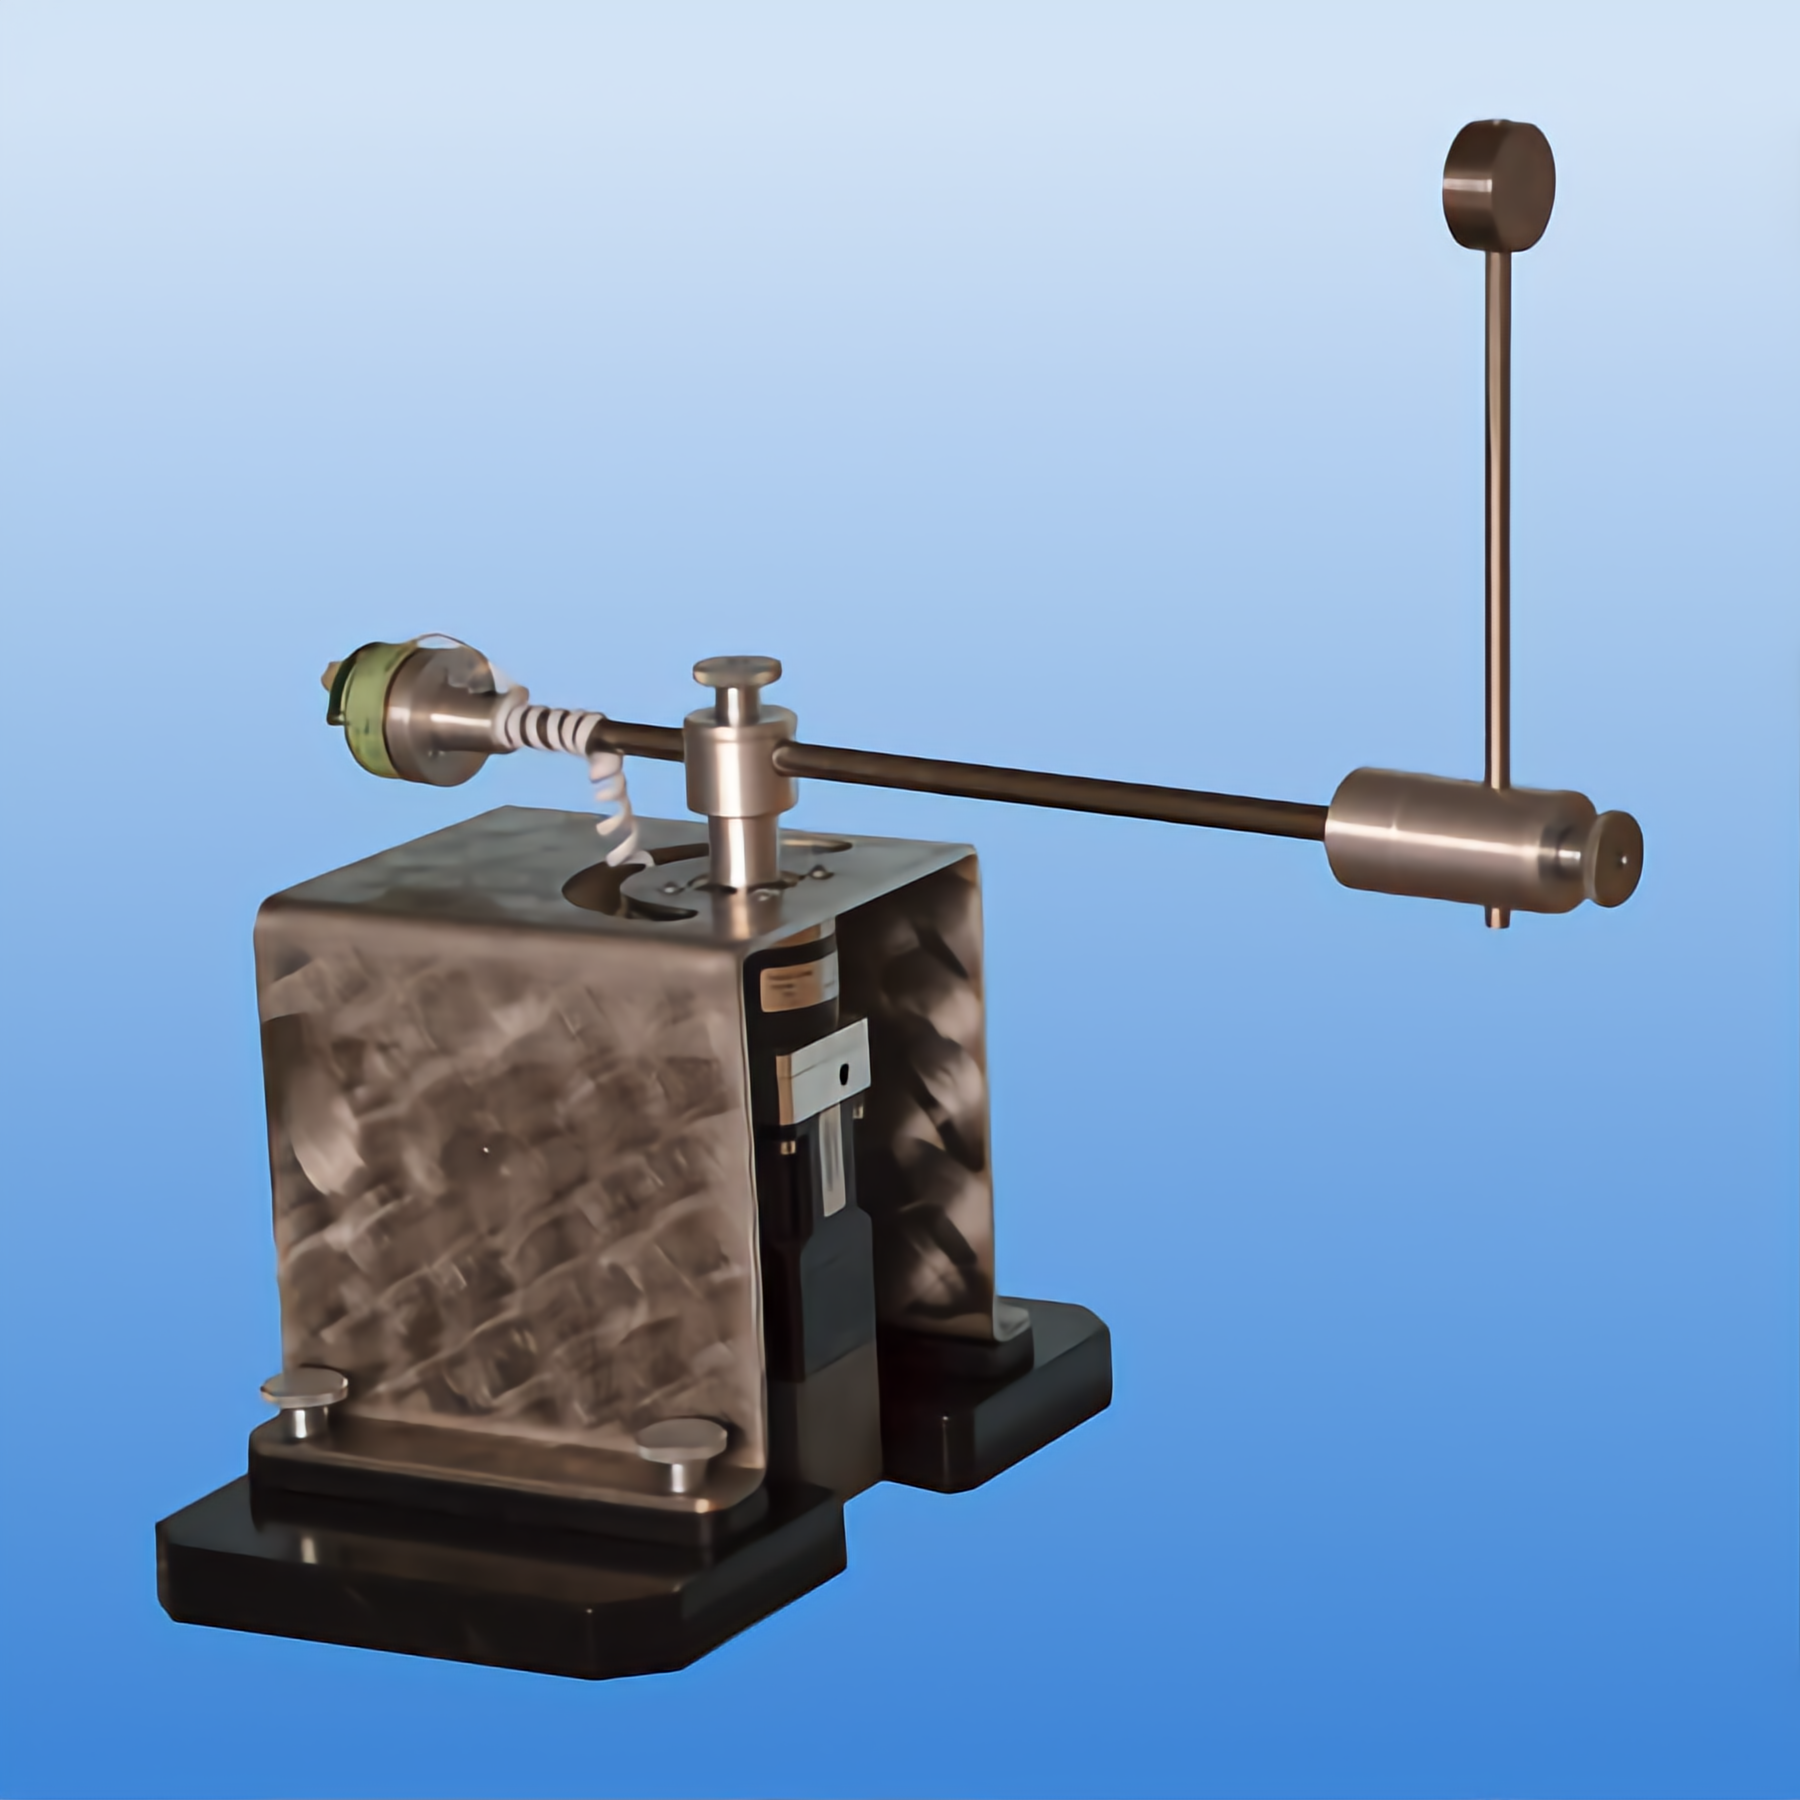
\includegraphics[width=.6\linewidth]{images/furutareal}
	\caption{Laboratory Furuta pendulum device}
	\label{furutareal}
\end{figure}
After measurements, the physical parameters of the device can be summarised in Tab.~\ref{furuta:values}.
\begin{table}[H]
	\caption{Values of Furuta Pendulum Parameters}
	\centering
\begin{tabular}{l l l}	
	\noalign{\hrule height 1pt}
	Parameter&Symbol&Value\\
	\noalign{\hrule height 1pt}
	Gravitational acceleration&$g$&\SI{9.81}{\metre\per\square\second}\\
	Mass of arm&$m_0$&\SI{0.6}{\kilogram}\\
	Mass of pendulum&$m_1$&\SI{0.198}{\kilogram}\\
	Length of arm&$L_0$&\SI{0.51}{\metre}\\
	Llength of pendulum&$L_1$&\SI{0.23}{\metre}\\
	Location of the pendulums center of mass&$l_1$&\SI{0.21}{\metre}\\
	Moment of inertia of arm&$I_0$& \SI{0.052}{\kilogram\per\square\metre}\\
	Moment of inertia of pendulum&$I_1$&\SI{8.72e-4}{\kilogram\per\square\metre}\\
	Sampling time&$\Ts$&\SI{0.02}{\second}\\
	\hline
\end{tabular}
\label{furuta:values}
\end{table}
By substituting values from Tab.~\ref{furuta:values} into \ref{linSSmodel:general} and evaluating it at the upright operation point 
\begin{equation}
\ui{x}{up} = \begin{bmatrix}0&0&0&0\end{bmatrix}^\intercal, 
\end{equation}
the linear, continuouss-time state-space model, representing the dynamic of the pendulum near the upright position is obtained
\begin{subequations}\label{linSSmodel:up}
	\begin{align}
	\ui{A}{c,up} &=\begin{bmatrix}
	0&1&\ 0& 0\\
	0&0&-15.8833&0\\
	0&0&\ 0&1\\
	0&0&\ \; \,77.5373&0
	\end{bmatrix},\\
	\ui{B}{c,up} &=\begin{bmatrix}
	\ 0\\
	\ \; \,17.6366\\
	\ 0\\
	-38.9393
	\end{bmatrix}.
	\end{align}
\end{subequations}
And with this model obtained, we are ready to proceed to controller design and pendulum control.
\section{Heuristic Swing-Up Control}
The first control Strategy is a Heuristic Swing-Up Control strategy. As was discussed in the respective part of the thesis (Section~\ref{Hswing:teoria}) it is a combined control strategy, where the control of the device is split into two phases initial excitation and stabilization of the pendulum. So the Heuristic Swing-Up Control will be developed in three steps. First is the development of the Energy-Shaping controller to excite the pendulum. Second is the development of a linear MPC to stabilize the pendulum. And the final step is to combine those two controllers to perform swing-up control of the pendulum.
\subsection{Energy-Shaping Controller}
In the first phase of control of the pendulum, the Energy-Shaping controller is used to swing the pendulum from the downside position into the upright position where the control of the process will be taken by another controller. 
Energy-Shaping controller can be designed by applying the control law (\ref{energy-shaping}) directly as a state-feedback controller.
\begin{figure}[H]
	\centering
\begin{subfigure}
	\centering
	% include first image
	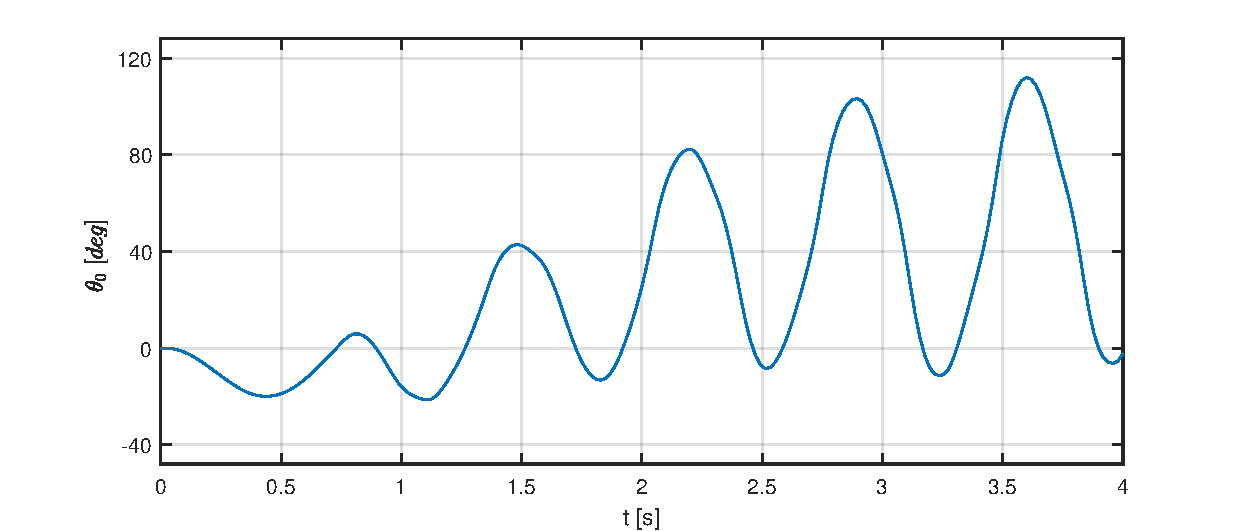
\includegraphics[scale=0.6]{images/swings/arm.pdf}  
\end{subfigure}
\begin{subfigure}
	\centering
	% include first image
	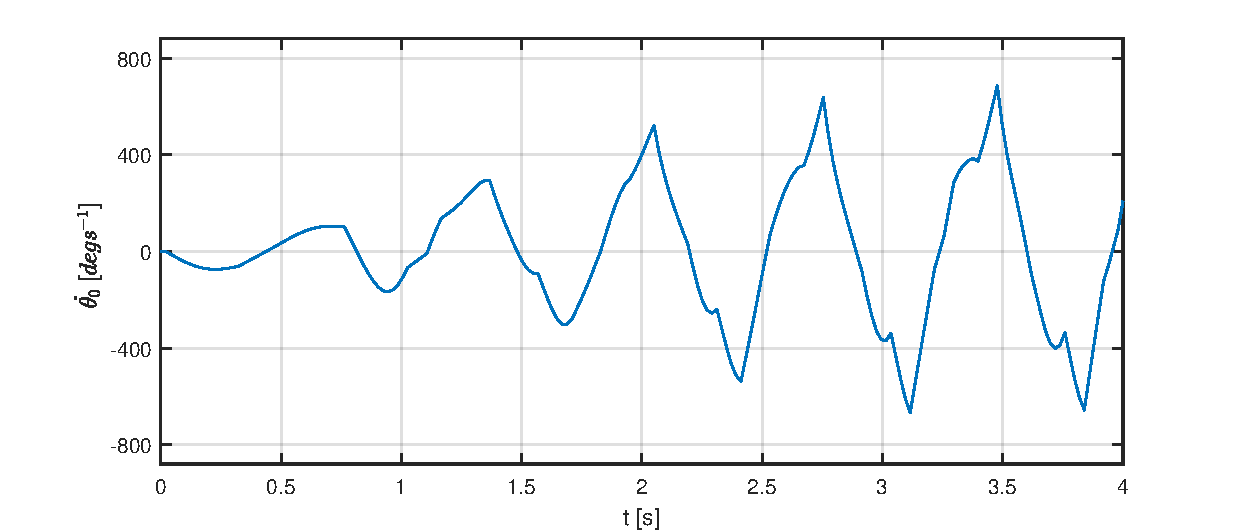
\includegraphics[scale=0.6]{images/swings/darm.pdf}  
\end{subfigure}
\begin{subfigure}
	\centering
	% include first image
	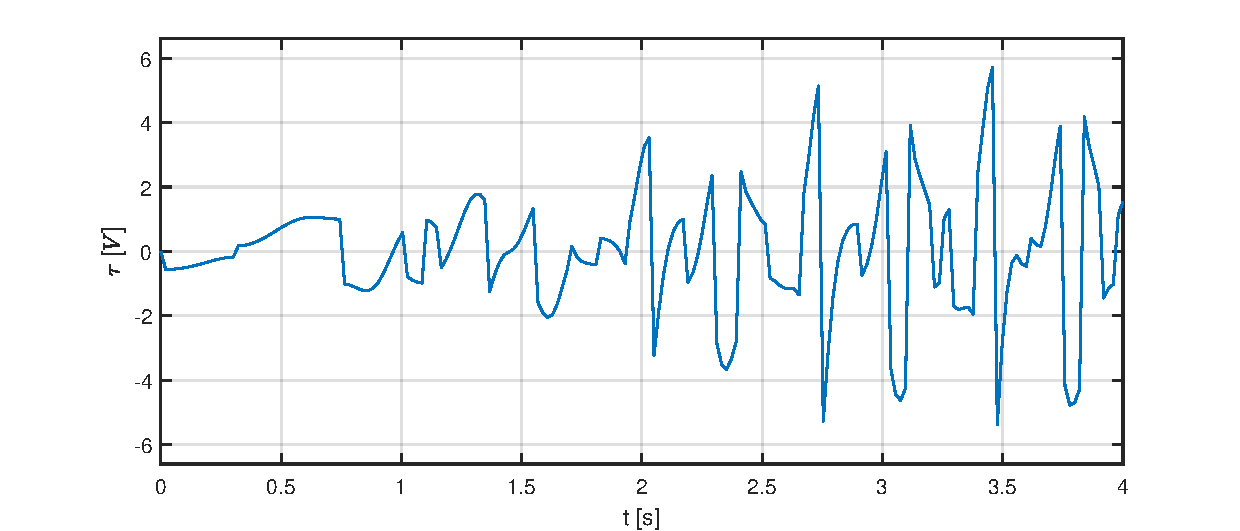
\includegraphics[scale=0.6]{images/swings/control.pdf}  
\end{subfigure}
	\caption{Control of the arm by the Energy-Shaping controller during the initial excitation scenario. The plots depict, respectively, the position of the arm $\theta_0(t)$, velocity of the arm $\dot{\theta}_0(t)$, and the control input $\tau(t)$.}
\label{swing}
\end{figure}
\begin{figure}[H]
	\centering
	\begin{subfigure}
		\centering
		% include first image
		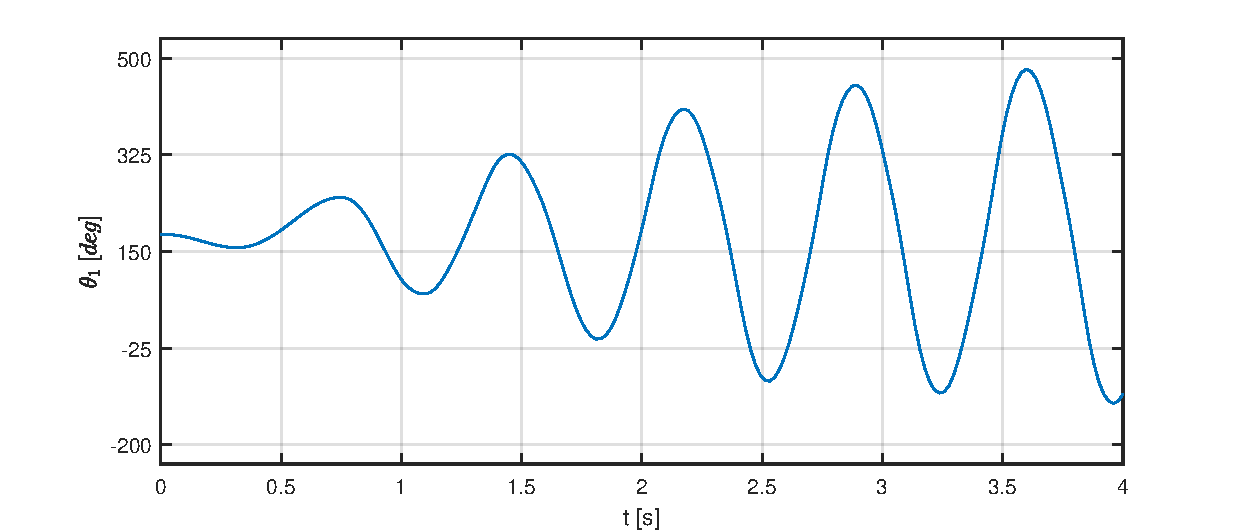
\includegraphics[scale=0.6]{images/swings/pend.pdf}  
	\end{subfigure}
	\begin{subfigure}
		\centering
		% include first image
		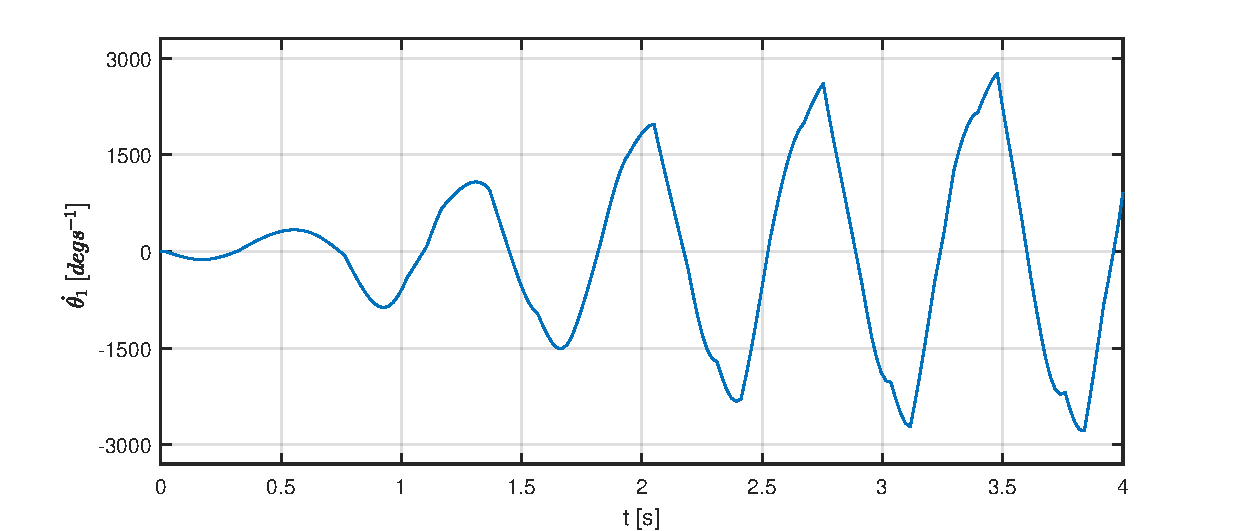
\includegraphics[scale=0.6]{images/swings/dpend.pdf}  
	\end{subfigure}
	\begin{subfigure}
		\centering
		% include first image
		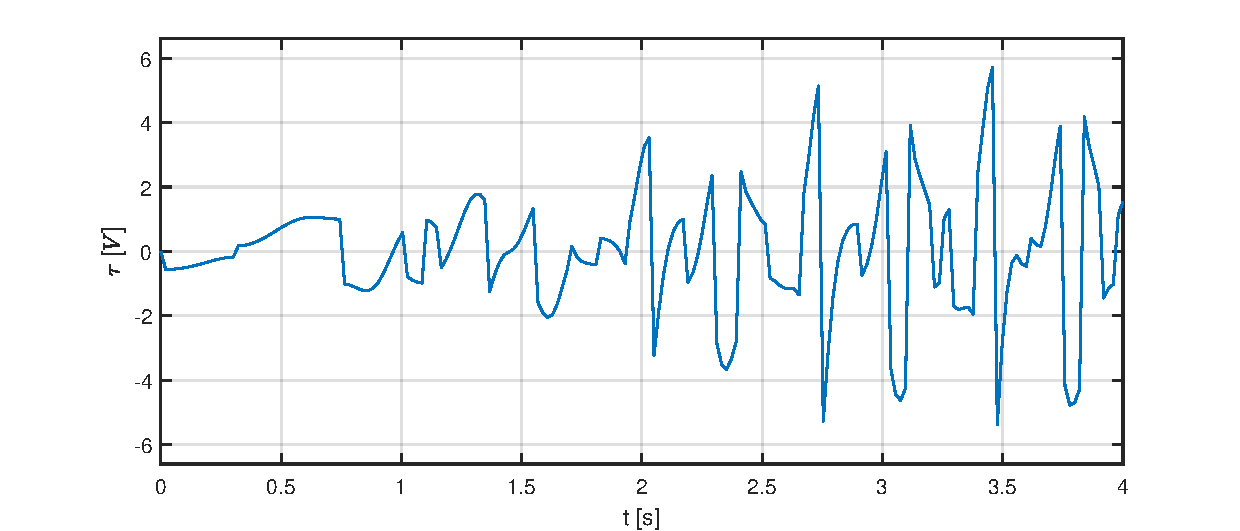
\includegraphics[scale=0.6]{images/swings/control.pdf}  
	\end{subfigure}
	\caption{Control of the pendulum by the Energy-Shaping controller during the initial excitation scenario. The plots depict, respectively, the position of the pendulum $\theta_1(t)$, velocity of the pendulum $\dot{\theta}_1(t)$, and the control input $\tau(t)$.}
	\label{swing1}
\end{figure}
\subsection{Model Predictive Control}
After the pendulum was brought in the vicinity of the upright operation point, it's furtherly controlled by a predictive controller. Due to the pendulums setup, the MPC formulation (\ref{mpcgeneral}) could be applied directly. As known, a linear MPC uses a linear prediction model \ref{linSSmodel:up} of the process to predict the behavior of the system over the prediction horizon. Such a predictive model is only relevant in vicinity of linearization point. That is the reason why the linear MPC strategy is used to conrol the pendulum only around upright position. 
The MPC is a discrete-time strategy, therefore the first step of the construction of such a controller is to obtain the discrete-time linear predictive model. Such model can be derived from continuous-time model (\ref{linSSmodel:up}) by some discretization method. In this thesis a zero-order hold method, with the discretization step, equal to devices sampling time, $\SI{0.02}{\second}$ is used. 
\begin{subequations}\label{dismatrices}
	\begin{align}
	\ui{A}{d} &=\begin{bmatrix}
	1&0.02&-0.0032& 0\\
	0&1&-0.3193&-0.0032\\
	0&0&\ \; \,1.0155&\ \; \,0.0201\\
	0&0&\ \; \,1.5588&\ \; \,1.0155
	\end{bmatrix},\\
	\ui{B}{d} &=\begin{bmatrix}
	\ \; \,0.0035\\
	\ \; \,0.3536\\
	-0.0078\\
	-0.7828
	\end{bmatrix}.\\
	\end{align}
\end{subequations}
The output matrices remain unchanged from (\ref{linmatrices}).\\ 

Now it is important to determine the range around the linearization point, where such a model is relevant. For that purpose will be evaluated the difference in outputs from the non-linear and linear model. For that purpose both models will be simulated with the same value of control input.
\begin{table}[H]
	\centering
	\caption{Comparisson of linear and non-linear models}
	\label{models:comparisson}
\begin{tabular}{c c}	
	\noalign{\hrule height 1pt}
	Initial angle of the pendulum [deg]&Difference in outputs [deg]\\
	\noalign{\hrule height 1pt}
	30&0.5977\\
	40&0.8370\\
	50&1.0200\\
	60&1.1474\\
	70&1.2314\\
	\hline
\end{tabular}
\end{table}
Those results demonstrate that an MPC can be used to control the pendulum roughly in $\pm50$deg around the upright position. Also, those results were obtained for the limit value of control input, for a smaller value of control input the difference, naturally, will be lesser.\\

The next, probably the most important, step is to design weight matrices $\ui{Q}{x}$ and $\ui{Q}{u}$. The main weights must be given to the position of the pendulum, what is our main controlled parameter, and the position of the arm, to prevent the possible scenario when the pendulum is stabilized at the upright position and the arm rotates constantly. 
\begin{equation}
\ui{Q}{x} = \begin{bmatrix}
10&0&0&0\\
0&0.08&0&0\\
0&0&10&0\\
0&0&0&0.2
\end{bmatrix}, \quad \ui{Q}{u} = 1.
\end{equation}
Weight matrices are the key point of MPC, as through them we define for MPC a requested control performance.
The remain MPC parametres can be set as shown in the following table
\begin{table}[H]
	\centering
	\caption{MPC parameters during the stabilization at the upright position}
	\begin{tabular}{l c c}
		\noalign{\hrule height 1pt}
		Parameter&Symbol&Value\\
		\noalign{\hrule height 1pt}
		Prediction horizon&$N$&$\ \; \,20$\\
		Initial condition&$x_0$&$\begin{bmatrix}0&0&0.5&-0.7\end{bmatrix}^\intercal$\\
		Constraint on control input-upper bound&$\ui{u}{max}$&$\ \; \,10$\\
		Constraint on control input-lower bound&$\ui{u}{min}$&$-10$\\
		\hline
	\end{tabular}
\end{table}
Due to the fact, that the Furuta pendulum performs a rotary motion, the safety constraints on the states are not necessary. So only present inequality constraints are the limit constraints on the control input.\\

Considering all aforesaid, the MPC formulation can be written in the following form
\begin{subequations}\label{mpc:linear}
	\begin{align}
	\min_{U}\ &\sum_{k=0}^{N-1} \lrp{\left\| \ui{Q}{x}x_{k}\right\|_2+\left\|\ui{Q}{u}u_{k}\right\|_2}\\
	\text{s.t.}\ &x_{k+1} = A_dx_{k} + B_du_{k}\qquad\qquad\ \ \,  k \in \mathbb{N}_0^{N-1}\\
	&x_0 = x(0)\\
	&\ui{u}{min}\leq u_{k}\leq \ui{u}{max}\qquad\qquad\qquad\;   k \in \mathbb{N}_0^{N-1}
	\end{align}
\end{subequations}
This predictive controller is designed in \textsc{MATLAB}, using the \textsc{YALMIP} toolbox \cite{YALMIP} to formulate the problem and \textsc{Gurobi} solver to solve it.
\begin{figure}[H]
	\centering
	\begin{subfigure}
		\centering
		% include first image
		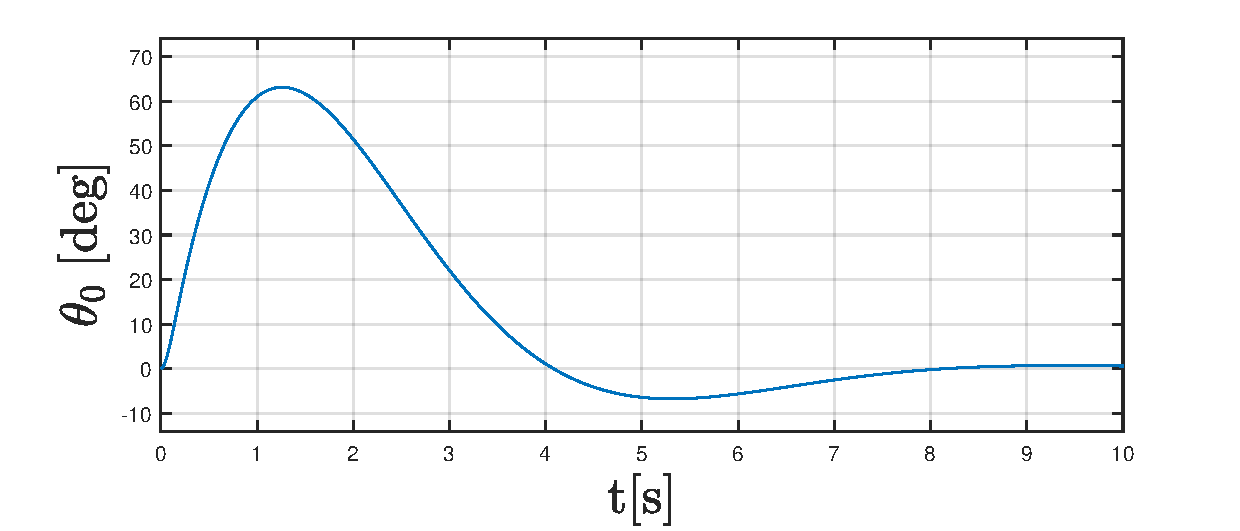
\includegraphics[scale=0.6]{images/MPC/arm.pdf}  
	\end{subfigure}
	\begin{subfigure}
		\centering
		% include first image
		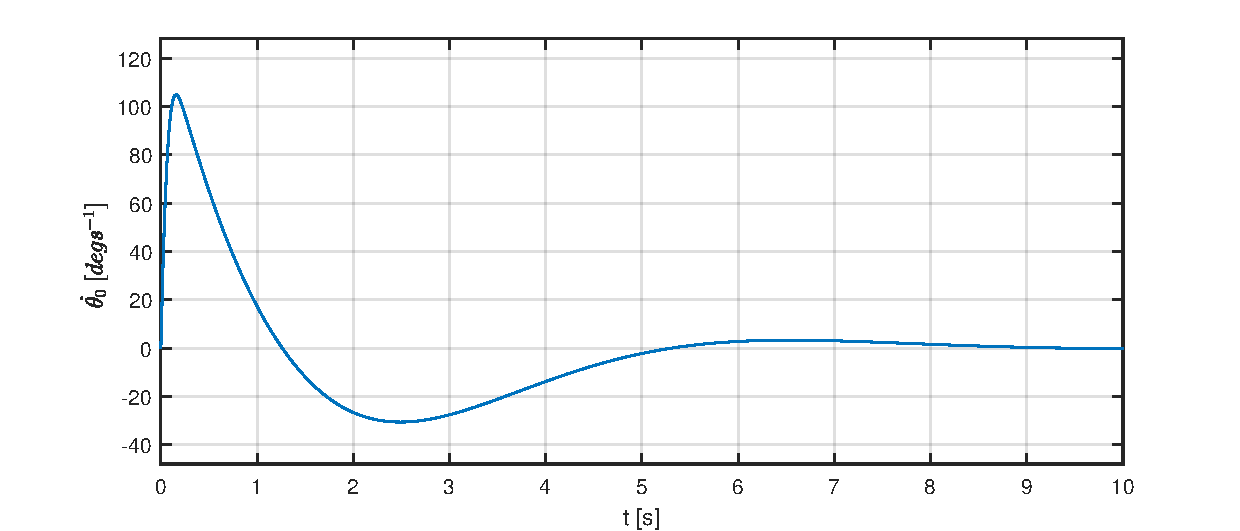
\includegraphics[scale=0.6]{images/MPC/darm.pdf}  
	\end{subfigure}
	\begin{subfigure}
		\centering
		% include first image
		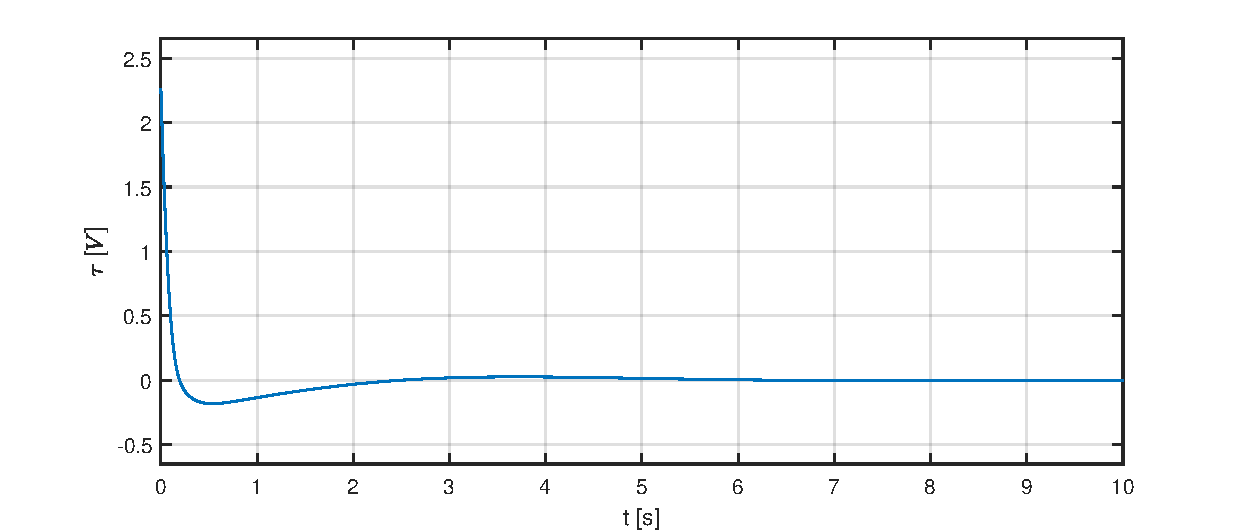
\includegraphics[scale=0.6]{images/MPC/control.pdf}  
	\end{subfigure}
	\caption{Control of the arm by the Model Predictive Controller during the stabilization scenario. The plots depict, respectively, the position of the arm $\theta_0(t)$, velocity of the arm $\dot{\theta}_0(t)$, and the control input $\tau(t)$.}
	\label{mpc}
\end{figure}
\begin{figure}[H]
	\centering
	\begin{subfigure}
		\centering
		% include first image
		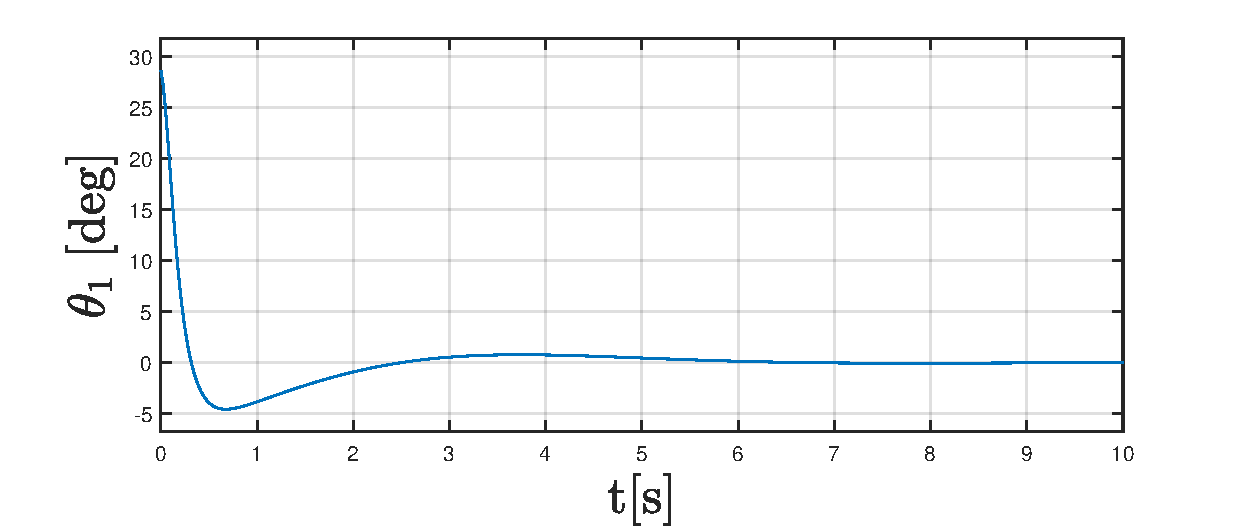
\includegraphics[scale=0.6]{images/MPC/pend.pdf}  
	\end{subfigure}
	\begin{subfigure}
		\centering
		% include first image
		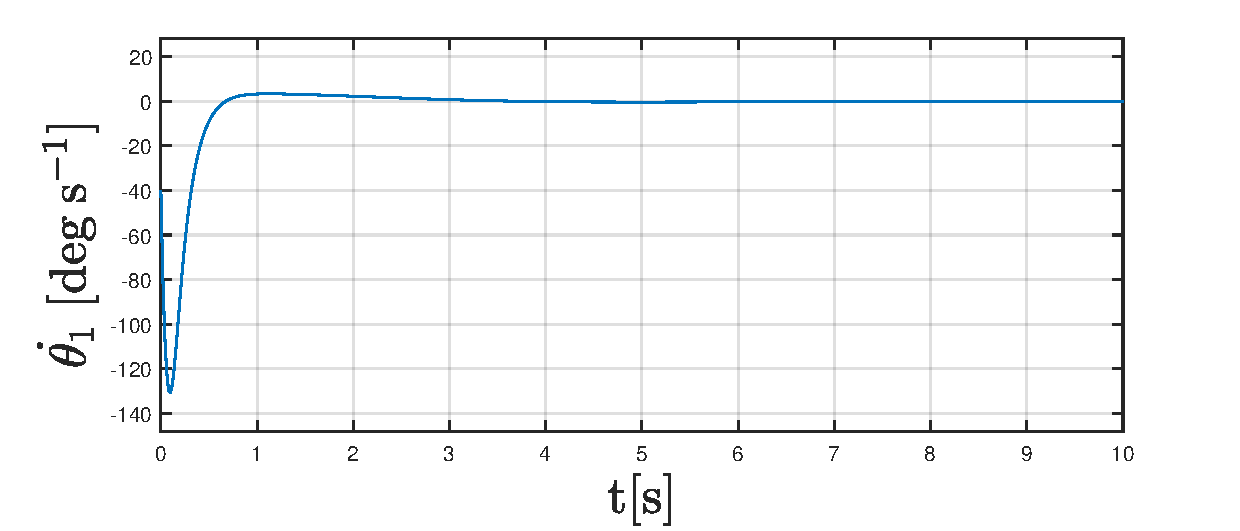
\includegraphics[scale=0.6]{images/MPC/dpend.pdf}  
	\end{subfigure}
	\begin{subfigure}
		\centering
		% include first image
		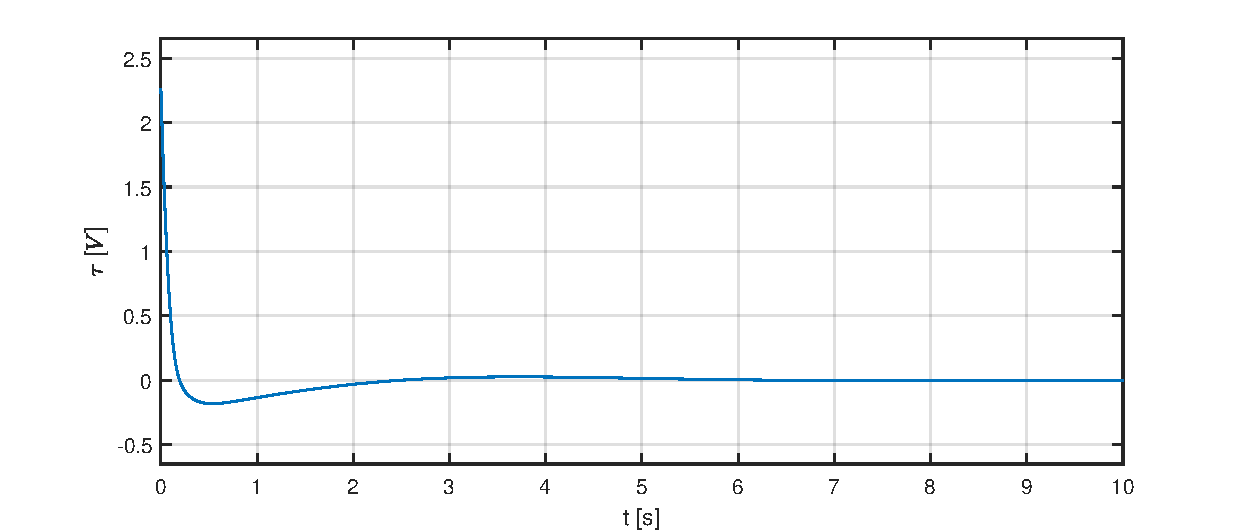
\includegraphics[scale=0.6]{images/MPC/control.pdf}  
	\end{subfigure}
	\caption{Control of the pendulum by the Model Predictive Controller during the stabilization scenario. The plots depict, respectively, the position of the pendulum $\theta_1(t)$, velocity of the pendulum $\dot{\theta}_1(t)$, and the control input $\tau(t)$.}
	\label{mpc1}
\end{figure}
\subsection{Combined Control Strategy}
To perform Swing-Up Control of the pendulum, a combined control strategy should be designed, because no MPC nor Swing-Up controller can not perform a Swing-Up control by itself. So the strategy of Heuristic Swing-Up Control is that at the beginning the pendulum is steady at the downside position and the Energy-Shaping controller is used to add the energy to the pendulum via its oscillation. As more energy is added to the pendulum, the greater the oscillations become. And as the pendulum is close to the upright operation point, the control law switches from Energy-Shaping to MPC, which finishes the Swing-Up Control by stabilizing the pendulum at the upright position.
\begin{figure}[H]
	\centering
	\begin{subfigure}
		\centering
		% include first image
		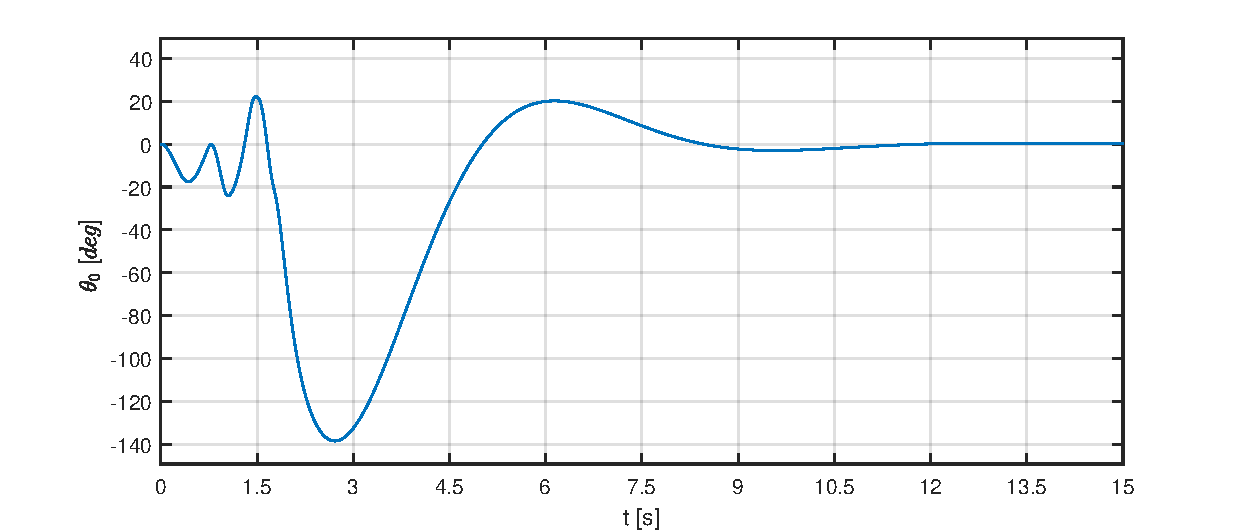
\includegraphics[scale=0.6]{images/Hswing/arm.pdf}  
	\end{subfigure}
	\begin{subfigure}
		\centering
		% include first image
		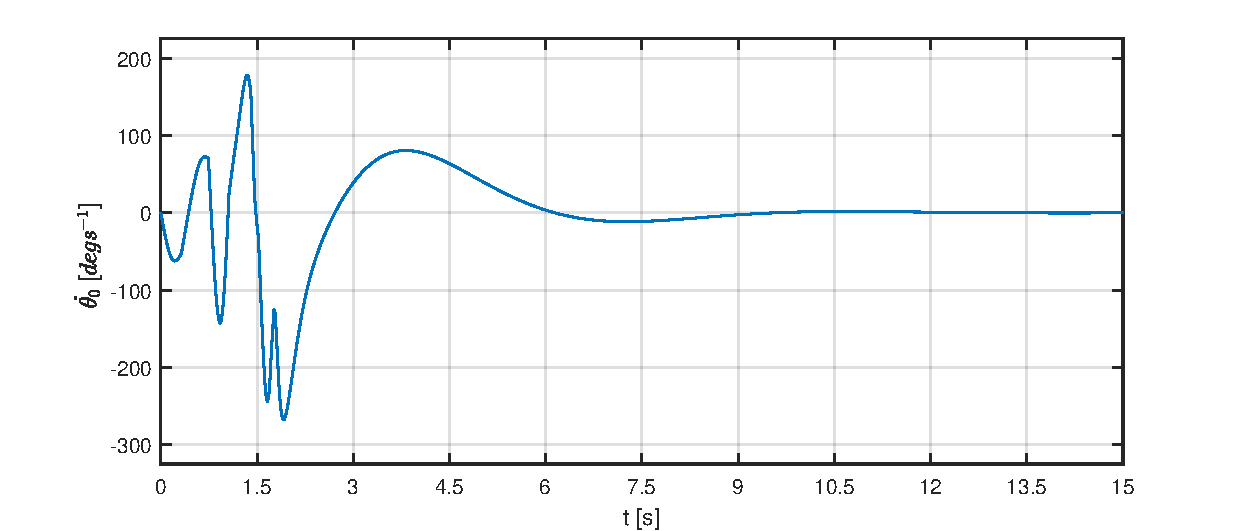
\includegraphics[scale=0.6]{images/Hswing/darm.pdf}  
	\end{subfigure}
	\begin{subfigure}
		\centering
		% include first image
		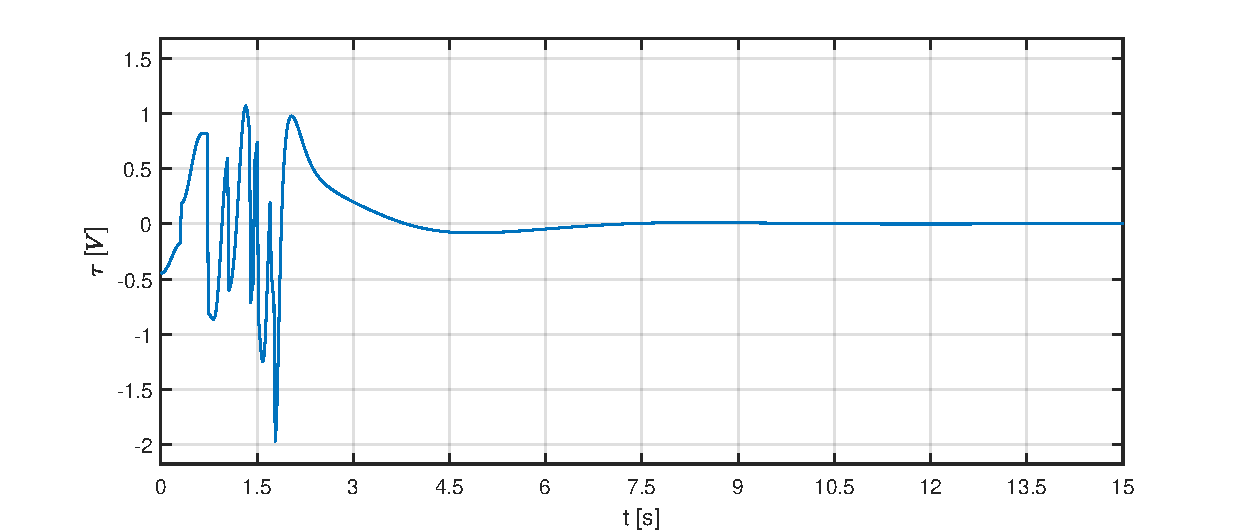
\includegraphics[scale=0.6]{images/Hswing/control.pdf}  
	\end{subfigure}
	\caption{Control of the arm during the Heuristic Swing-Up scenario. The plots depict, respectively, the position of the arm $\theta_0(t)$, velocity of the arm $\dot{\theta}_0(t)$, and the control input $\tau(t)$.}
	\label{combo}
\end{figure}
\begin{figure}[H]
	\centering
	\begin{subfigure}
		\centering
		% include first image
		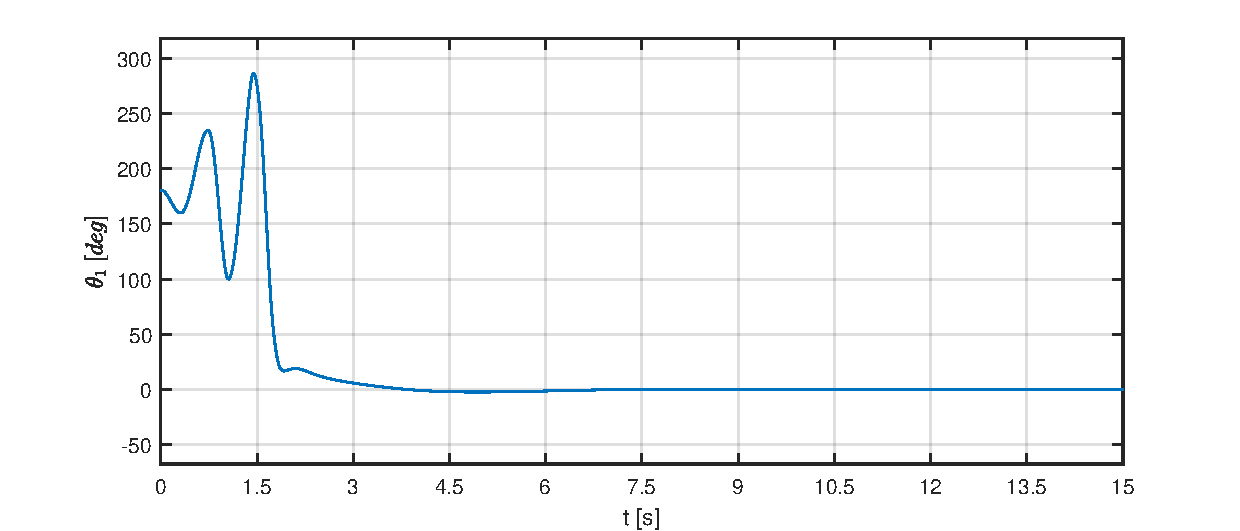
\includegraphics[scale=0.6]{images/Hswing/pend.pdf}  
	\end{subfigure}
	\begin{subfigure}
		\centering
		% include first image
		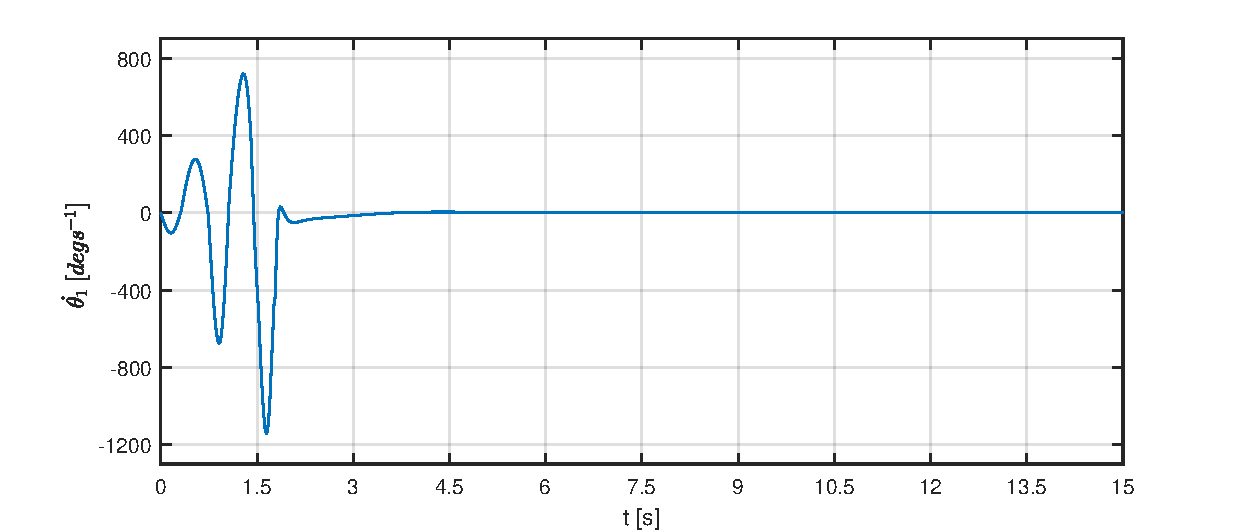
\includegraphics[scale=0.6]{images/Hswing/dpend.pdf}  
	\end{subfigure}
	\begin{subfigure}
		\centering
		% include first image
		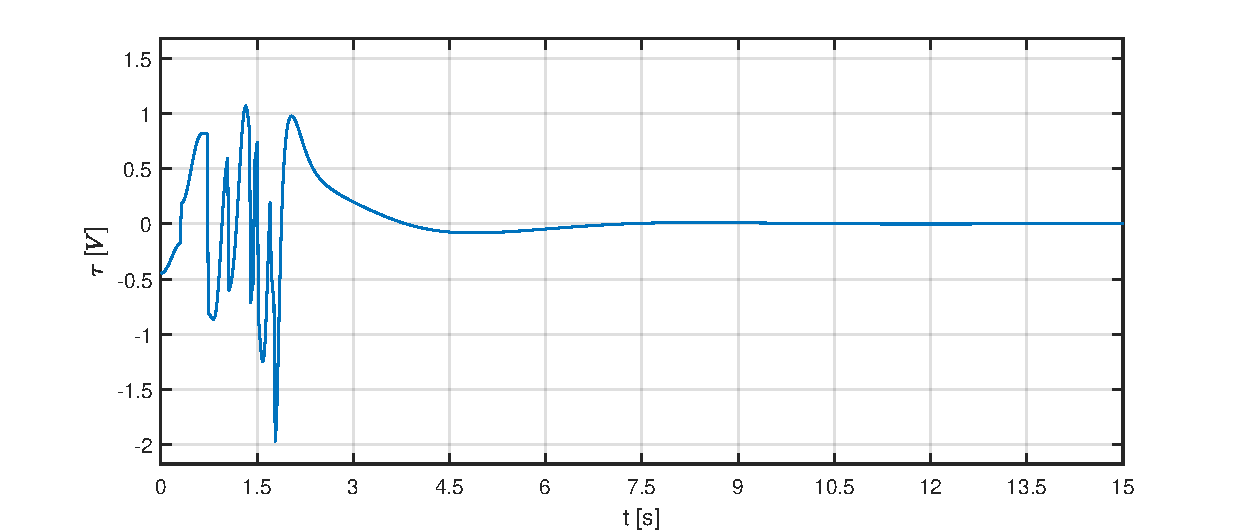
\includegraphics[scale=0.6]{images/Hswing/control.pdf}  
	\end{subfigure}
	\caption{Control of the pendulum during the Heuristic Swing-Up scenario. The plots depict, respectively, the position of the pendulum $\theta_1(t)$, velocity of the pendulum $\dot{\theta}_1(t)$, and the control input $\tau(t)$.}
	\label{combo1}
\end{figure}
\section{Optimal Swing-Up Control}
The last control strategy is an Optimal Swing-Up Control. In this strategy, only one non-linear Model Predictive Controller (NMPC) is used to perform both the swing-up and the stabilization of the pendulum. Such control performance is possible due to the fact that in NMPC the non-linear model (\ref{nonlinmodel}) is used to predict the future evolution of the process.  Usage of this non-linear model, leads to a Non-linear Programing (NLP) problem, and solving a NLP problem is ot a trivial process. In this work a \textsc{MATMPC} toolbox is used \cite{MATMPC} to formulate and solve this problem.\\

A NMPC problen can be formulated in a similar form as linear MPC problem (\ref{mpc:linear}):
\begin{subequations}\label{nmpcgeneral}
	\begin{align}
	\min_{U}\ &\sum_{k=0}^{N-1} \lrp{ x_{k}^\intercal\ui{Q}{x}x_{k}+u_{k}^\intercal\ui{Q}{u}u_{k}}\\
\text{s.t.}\ &x_{k+1} = f(x_{k}, u_{k})\qquad\qquad\qquad \ \   k \in \mathbb{N}_0^{N-1}\label{eq3.6b}\\
&x_0 = x(0)\\
&\ui{u}{min}\leq u_{k}\leq \ui{u}{max}\qquad\qquad\qquad\;   k \in \mathbb{N}_0^{N-1}
	\end{align}
\end{subequations}
Tho only difference is in equality constraint (\ref{eq3.6b}), where instead of linear model (\ref{linSSmodel:up}) a non-linear dynamic model (\ref{mpc:linear}) is used. The presense of the non-linear constraint makes this optimization problem a Nonlinear Programming (NLP) problem. The way to solve the general NLP problem was described in Section~\ref{nmpcsection}. 
The rules for weight matrices in NMPC strategy are similar to those, used in linear MPC, except that to the arm must be given more freedom and we are willing to invest more into control inputs. It's because of that the controller must not only stabilize the pendulum but also perform a swing-up.
\begin{equation}\label{NMPC:weights}
\ui{Q}{x} = \begin{bmatrix}
1&0&0&0\\
0&0.1&0&0\\
0&0&3&0\\
0&0&0&0.1
\end{bmatrix}, \quad \ui{Q}{u} = 0.1.
\end{equation}
Other NMPC parameters are shown in the following table
\begin{table}[H]
	\centering
	\caption{NMPC parameters for the Optimal Swing-Up Control strategy}
	\begin{tabular}{l c c}
		\noalign{\hrule height 1pt}
		Parameter&Symbol&Value\\
		\noalign{\hrule height 1pt}
		Prediction horizon&$N$&$20$\\
		Initial condition&$x_0$&$\begin{bmatrix}0,0,\pi,0\end{bmatrix}^\intercal$\\
		Constraint on control input-upper bound&$\ui{u}{max}$&$\ \; \,10$\\
		Constraint on control input-lower bound&$\ui{u}{min}$&$-10$\\
		\hline
	\end{tabular}
\end{table}
The parameters are similar, that were used in MPC, except for the initial condition, that in case of NMPC the pendulum's steady downside position.\\

Now, as the rules for the NMPC are defined, we can proceed to the controller design itself, using a \textsc{MATMPC} toolbox. From a user perspective, the design of such an NMPC strategy, usage of \textsc{MATMPC} toolbox is trivial. You only have to set the NMPC parameters and define a prediction model (\ref{nonlinmodel}). Then, the \textsc{MATMPC} toolbox will automatically construct and solve the following NLP problem
\begin{subequations}\label{NLP}
	\begin{align}
	\min_{X,\,U}\ \frac{1}{2}&\sum_{k=0}^{N-1} (\left\| h_k(x_k, u_k)\right\|_2\ui{Q}{k}) + \frac{1}{2}\left\|h_N(x_N)\right\|_2\ui{Q}{N}\label{NLP:obj}\\
	\text{s.t.}\quad &x_{k+1} = \phi_k(x_{k},u_{k})\qquad\qquad\qquad\, k \in \mathbb{N}_0^{N-1}\label{NLP:model}\\
	&x_0 = x(0)\\
	&\ui{u}{min}\leq u_{k}\leq \ui{u}{max}\qquad\qquad\qquad\;   k \in \mathbb{N}_0^{N-1}	
	\end{align}
\end{subequations}
There are a couple of things about such formulation, which have to be highlighted. First of all, the objective function. Here, unlike the other formulations, the vectors of optimized states and controls $X$ and $U$ are not part of the objective function directly, but they are represented by a vector function $h_k(x, u)$. Also the predicted states for the stage $N$, represented by $h_N(x_N)$, are present in the function. Next, the continuity constraint (\ref{NLP:model}). It supposes to represent the prediction model. However, instead of using a non-linear dynamic model of the pendulum,  a numerical integration operator $\phi_k(x_{k},u_{k})$,that solves the following initial value problem (IVP) and returns the solution at $t_{k+1}$, is used. 
\begin{equation}
0=f\lrp{\dot{x}(t), x(t),u(t),t},\quad x(0)=x_k.
\end{equation}
where $\dot{x}(t)$ is a non-linear dynamic model of the process (\ref{nonlinmodel}).

Matrices $\ui{Q}{k}$ and $\ui{Q}{N}$ are the weights for each term for stage $k$. As the weight matrix $\ui{Q}{k}$ meets the function $h_k(x, u)$, it has to have the proper size of $n_x+n_u\times N$. And the weight matrix $\ui{Q}{N}$ has the size of $n_x\times 1$, where $n_x$ is a number of states and $n_u$ is the number of control inputs. Matrix $\ui{Q}{k}$ can by designed by extending the NMPC weight matrix $\ui{Q}{x}$ by a weight of control input. And the matrix $\ui{Q}{N}$ is the same as $\ui{Q}{x}$.
\begin{equation}\label{NLP:weights}
\ui{Q}{k} = \begin{bmatrix}
				1&0&0&0&0\\
				0&0.1&0&0&0\\
				0&0&3&0&0\\
				0&0&0&0.1&0\\
				0&0&0&0&0.1
			\end{bmatrix}, \quad 
\ui{Q}{N} = \begin{bmatrix}
				1&0&0&0\\
				0&0.1&0&0\\
				0&0&3&0\\
				0&0&0&0.1
			\end{bmatrix}.
\end{equation}
With this setup the \textsc{MATMPC} toolbox solves the listed above NLP, using the Sequential Quadratic Programming (SQP) method, which was described in the corresponding part of the thesis - Section~\ref{SQP:theory}. Also, additional software must be installed:
\begin{itemize}
	\item \textbf{CasAdi} - to obtain the needed derivatives to perform optimization (\url{https://github.com/casadi/casadi/wiki}).
	\item \textbf{MinGW-w64 C/C++ Compiler} - to compile \textsc{MATMPC} modules into MEX functions with performance comparable to plain C/C++ solvers.
\end{itemize}
And with such setup, a Optimal Swing-Up control of the Pendulum can be performed.
\newpage
\begin{figure}[H]
	\centering
	\begin{subfigure}
		\centering
		% include first image
		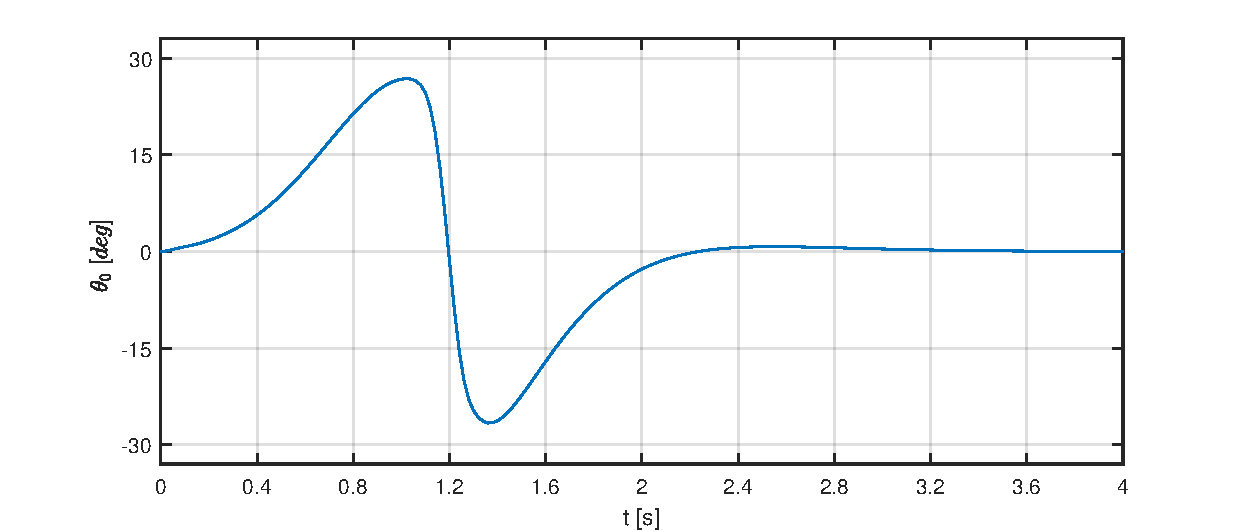
\includegraphics[scale=0.6]{images/Oswing/arm.pdf}  
	\end{subfigure}
	\begin{subfigure}
		\centering
		% include first image
		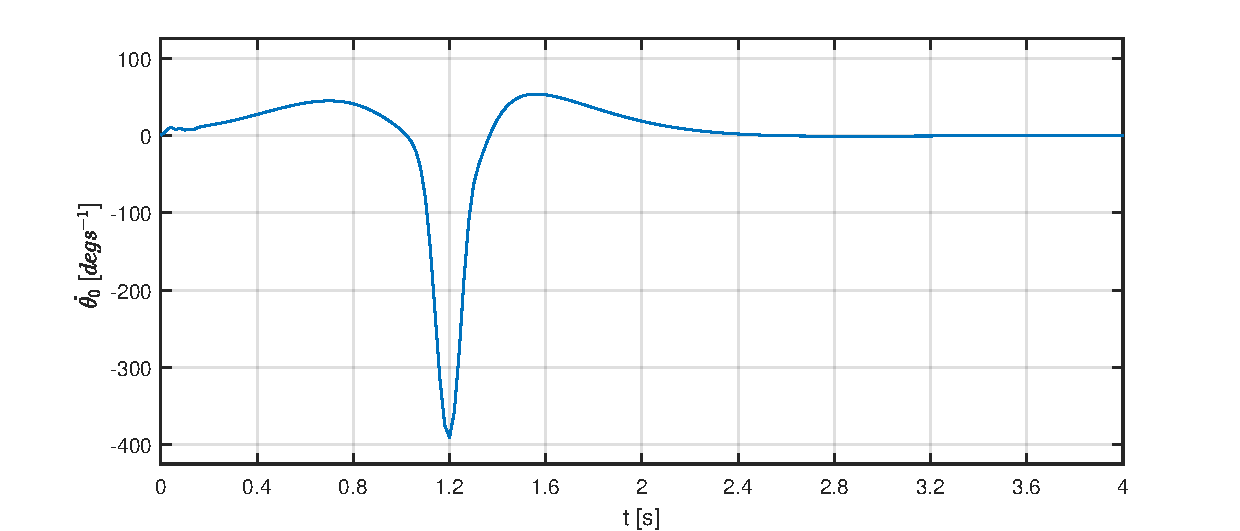
\includegraphics[scale=0.6]{images/Oswing/darm.pdf}  
	\end{subfigure}
	\begin{subfigure}
		\centering
		% include first image
		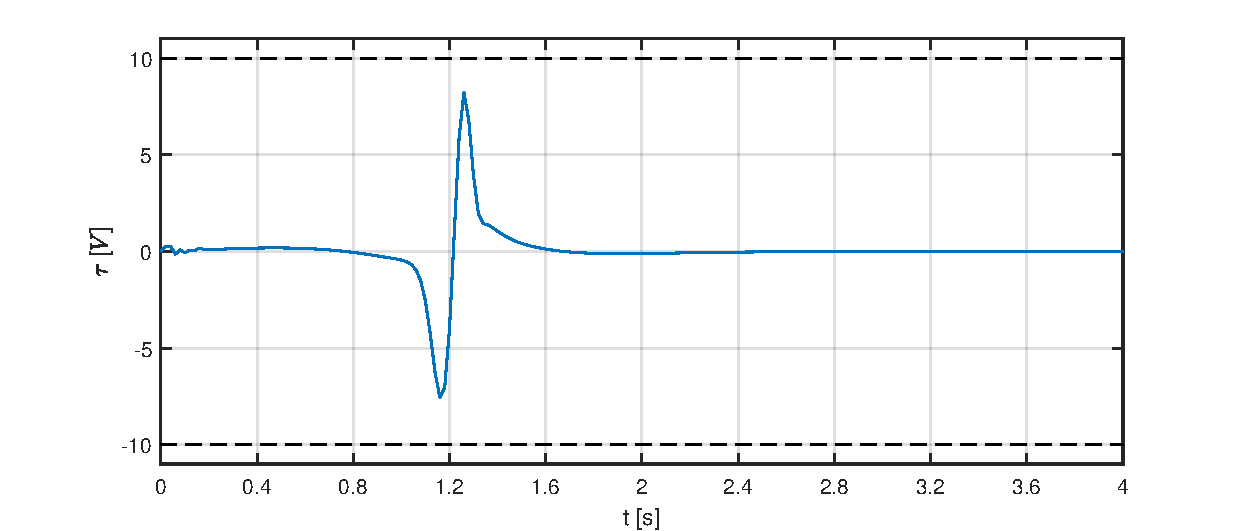
\includegraphics[scale=0.6]{images/Oswing/control.pdf}  
	\end{subfigure}
	\caption{Control of the arm during the Optimal Swing-Up scenario. The plots depict, respectively, the position of the arm $\theta_0(t)$, velocity of the arm $\dot{\theta}_0(t)$, and the control input $\tau(t)$.}
	\label{NMPC:results}
\end{figure}
\begin{figure}[H]
	\centering
	\begin{subfigure}
		\centering
		% include first image
		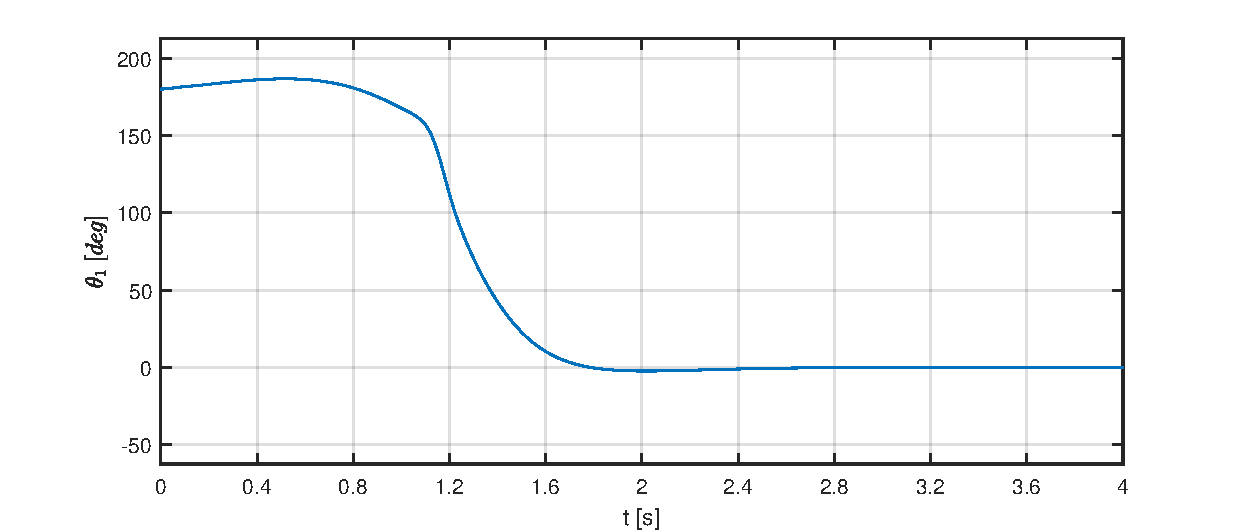
\includegraphics[scale=0.6]{images/Oswing/pend.pdf}  
	\end{subfigure}
	\begin{subfigure}
		\centering
		% include first image
		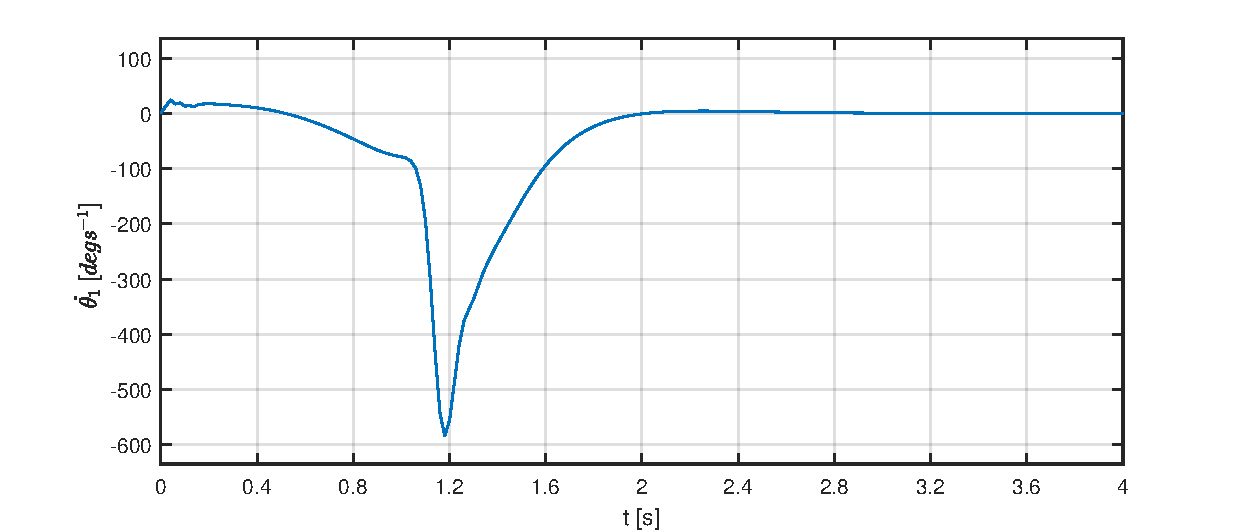
\includegraphics[scale=0.6]{images/Oswing/dpend.pdf}  
	\end{subfigure}
	\begin{subfigure}
		\centering
		% include first image
		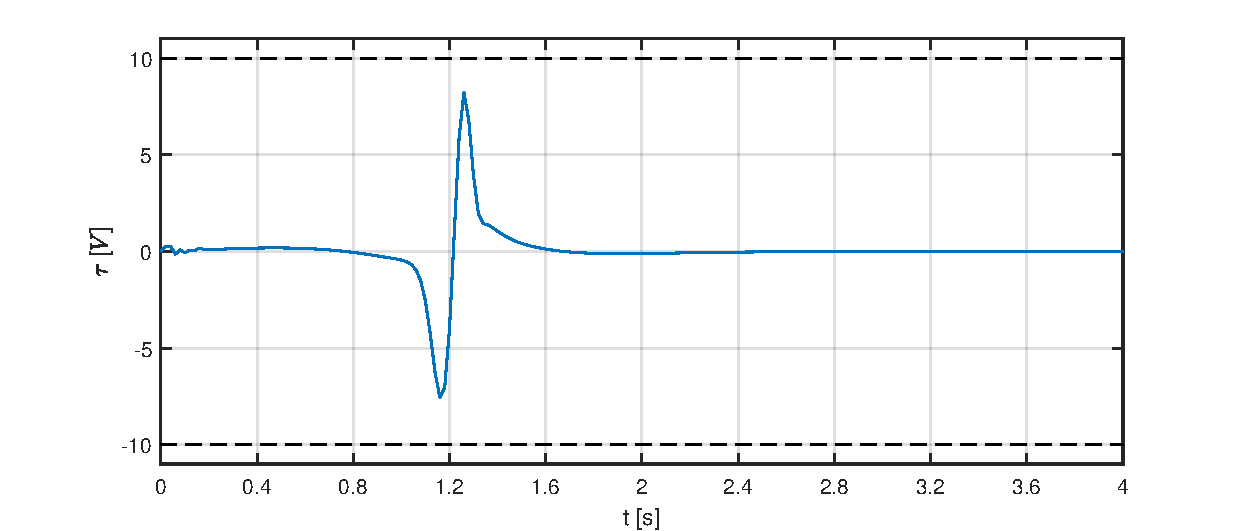
\includegraphics[scale=0.6]{images/Oswing/control.pdf}  
	\end{subfigure}
	\caption{Control of the pendulum during the Optimal Swing-Up scenario. The plots depict, respectively, the position of the pendulum $\theta_1(t)$, velocity of the pendulum $\dot{\theta}_1(t)$, and the control input $\tau(t)$.}
	\label{NMPC:results1}
\end{figure}
Considering the results in Fig.~\ref{NMPC:results} and Fig.~\ref{NMPC:results1} we can conclude, that a non-linear predictive controller was designed correctly. It's capable to perform the Swing-Up control of the pendulum with its stabilization at the upright position without constraints violation. Also, the control was performed in an impressive time of $\SI{2.5}{\second}$.
\section{Discussion About Results}
The first control strategy was the Heuristic Swing-Up Control strategy. The simulation results of controlling the pendulum by this strategy are shown in Fig.\ref{mpc}. As can be observed, both used controllers are designed correctly and capable to perform the swing-up control of the pendulum. \\

The second control strategy was the Optimal Swing-Up Control strategy. Considering the results in Fig.~\ref{NMPC:results} we can conclude, that the Optimal Swing-Up Control strategy was developed correctly and a non-linear predictive controller was tuned properly. As it's capable to perform the Swing-Up control of the pendulum with only one swing of the pendulum. Also, the control was performed in an impressive time of $\SI{2.5}{\second}$.\\

Now the question is, which control strategy is better. To answer that question, we compare the quality of controlled responses for the Heuristic and Optimal Swing-Up control strategies. Here, we evaluate the settling time for the pendulum stabilization, integral abslolute error (IAE) and MPC problem solving time.
\begin{table}[h]
	\centering
	\caption{Comparison of Heuristic and Optimal Swing-Up control strategies}
	\begin{tabular}{l c c c c c}
		\noalign{\hrule height 1pt}
		\multirow{2}{*}{Strategy}&\multirow{2}{*}{Settling Time}&\multirow{2}{*}{IAE}&\multicolumn{3}{c}{Solving Time}\\
		&&&$\ui{t}{min}$&$\ui{t}{avg}$&$\ui{t}{max}$\\
		\noalign{\hrule height 1pt}
		Heuristic Swing-Up&7.51&304.81&0.0156&0.0234&0.0313\\
		Optimal Swing-Up&3.2&205.56&0.0313&0.0469&0.0625\\
		\hline
	\end{tabular}
\end{table}
Settling time and IAE are evaluated for the control of the pendulum's position $\theta_1$, as it is the main controlled objective. Also, the control performance is visualized on the following graphs.
\newpage
\begin{figure}[H]
	\centering
	\begin{subfigure}
		\centering
		% include first image
		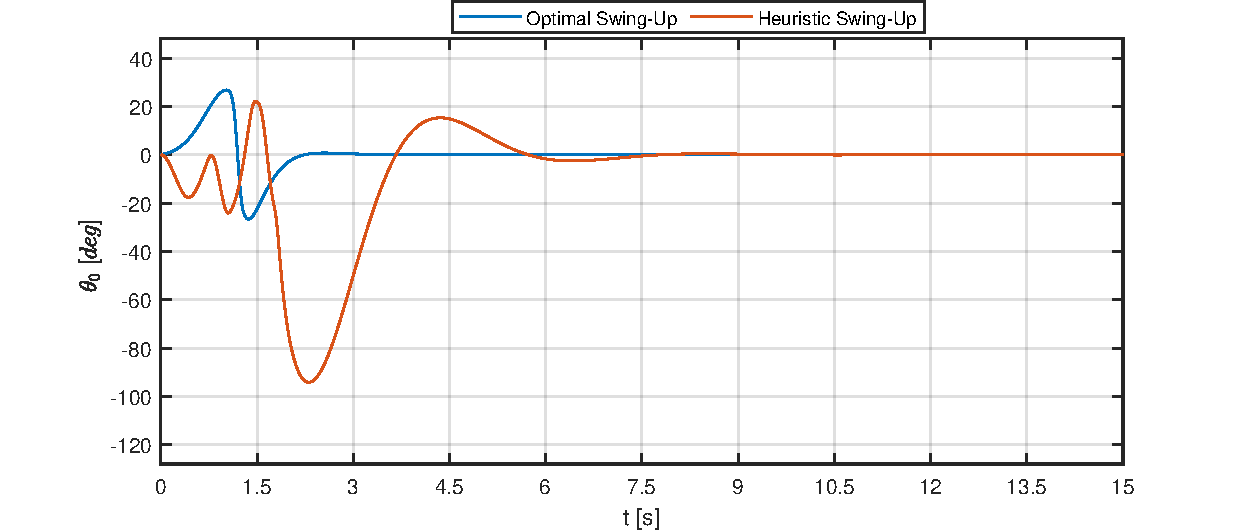
\includegraphics[scale=0.6]{images/Dswing/arm.pdf}  
	\end{subfigure}
	\begin{subfigure}
		\centering
		% include first image
		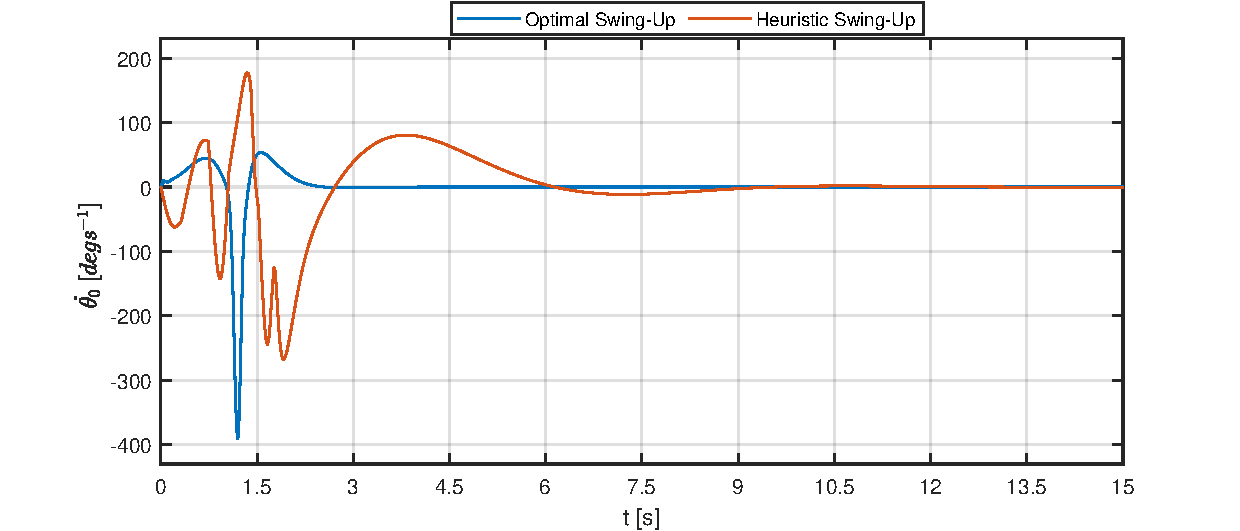
\includegraphics[scale=0.6]{images/Dswing/darm.pdf}  
	\end{subfigure}
	\begin{subfigure}
		\centering
		% include first image
		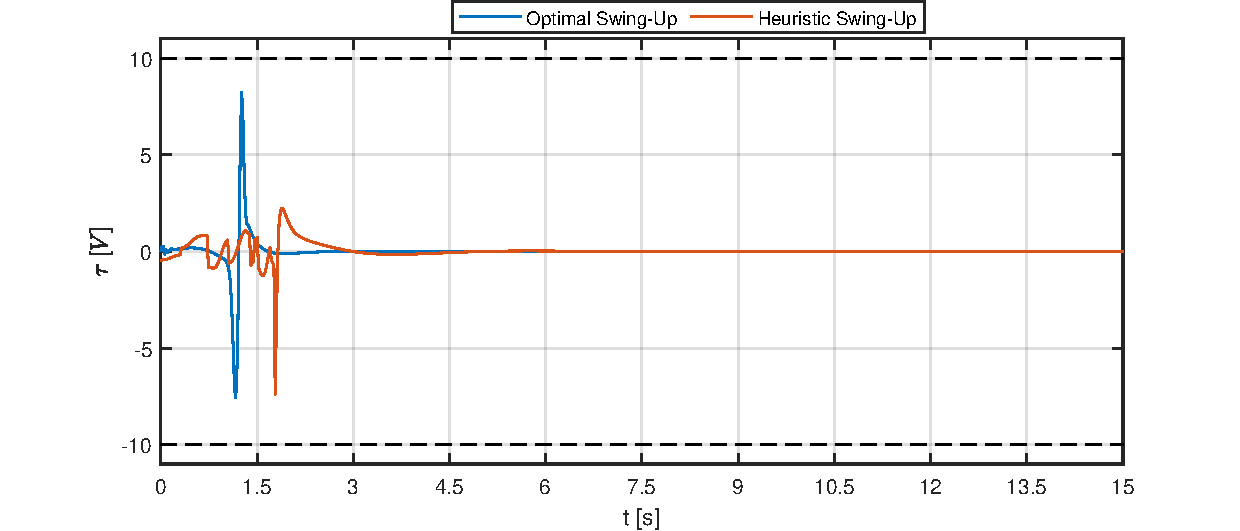
\includegraphics[scale=0.6]{images/Dswing/control.pdf}  
	\end{subfigure}
	\caption{Comparison of the arm control arm during by the Optimal and heuristic Swing-Up control strategies. The plots depict, respectively, the position of the arm $\theta_0(t)$, velocity of the arm $\dot{\theta}_0(t)$, and the control input $\tau(t)$.}
	\label{results}
\end{figure}
\begin{figure}[H]
\centering
\begin{subfigure}
	\centering
	% include first image
	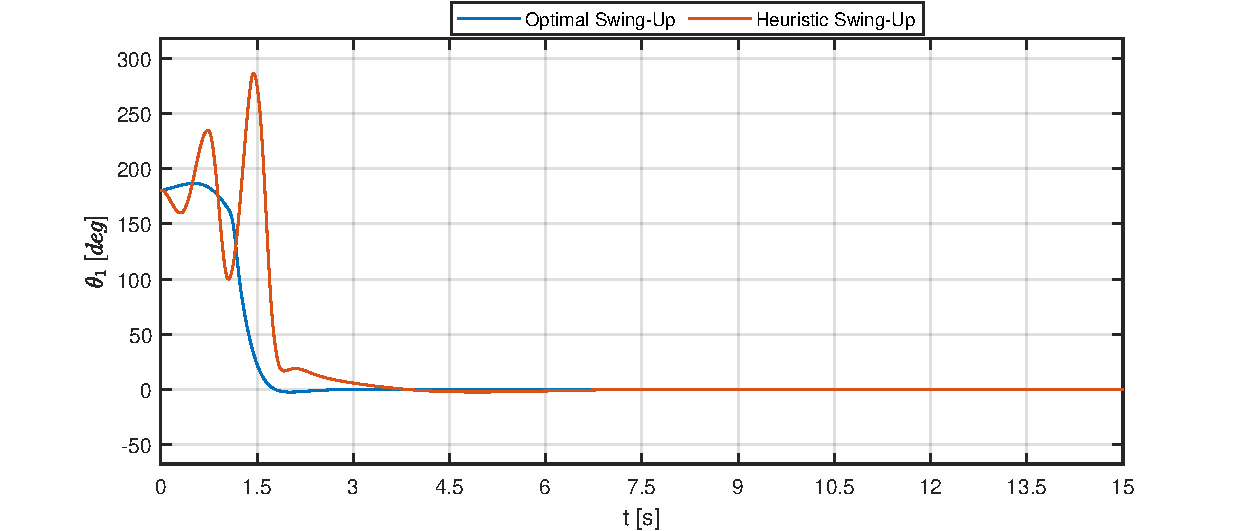
\includegraphics[scale=0.6]{images/Dswing/pend.pdf}  
\end{subfigure}
\begin{subfigure}
	\centering
	% include first image
	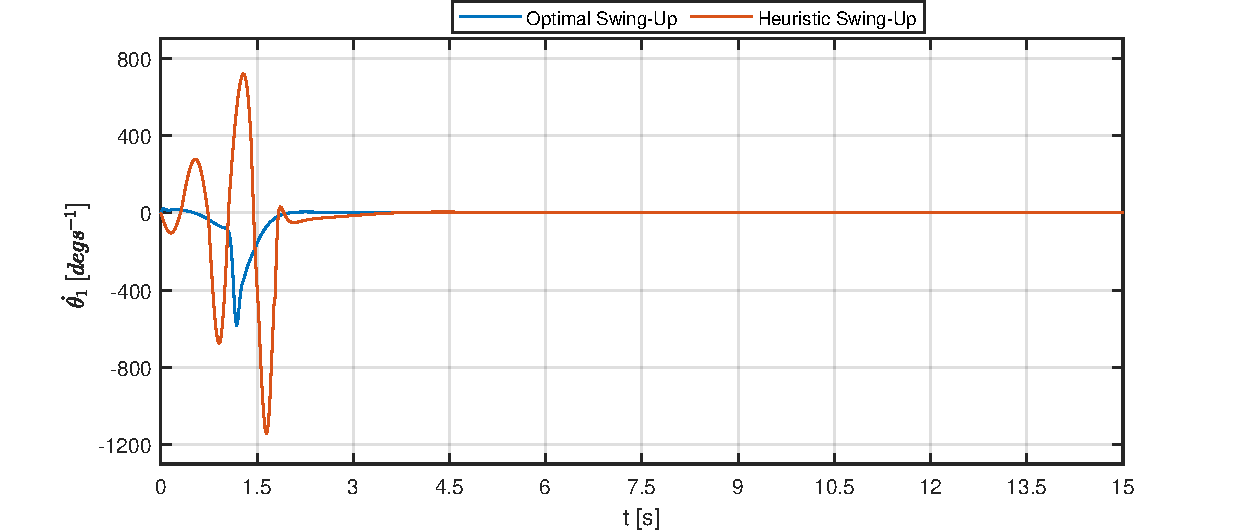
\includegraphics[scale=0.6]{images/Dswing/dpend.pdf}  
\end{subfigure}
\begin{subfigure}
	\centering
	% include first image
	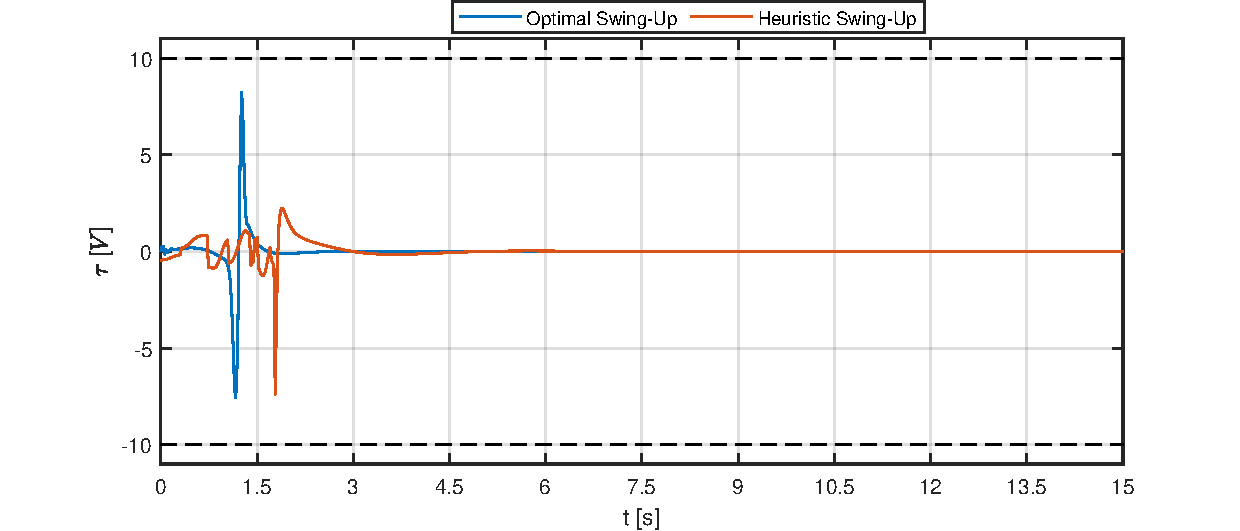
\includegraphics[scale=0.6]{images/Dswing/control.pdf}  
\end{subfigure}
\caption{Comparison of the arm control arm during by the Optimal and Heuristic Swing-Up control strategies. The plots depict, respectively, the position of the pendulum $\theta_1(t)$, velocity of the pendulum $\dot{\theta}_1(t)$, and the control input $\tau(t)$.}
\label{results1}
\end{figure}
Based on the IAE and regulation time, the  Optimal Swing-Up control strategy shows much better control performance. It also regulates the position of the arm $\theta_0$ to the origin much faster than the Heuristic Swing-Up control strategy. But it is much more expensive both in software, as it requires a \textsc{MATMPC} toolbox, CasADi tool, C/C++ compiler, and hardware, as it requires a stronger computation machine to achieve a comparable solving time of optimization problem. Also, neither of the strategies were able to solve an optimization problem under the sampling time. From my point of view, the most obvious solution to that problem is a hardware upgrade, as the simulations were performed on a much-used laptop.